\section{Proposed Architecture} \label{arch}

\subsubsection{Overview}

TorCoin runs as a standalone service, and requires no modification of the core Tor codebase. The system can be broken into four components, which share code across clients and relays, but behave differently depending on role. Figure 3.1 shows a basic overview of their architecture.

\begin{figure}
  \centering
    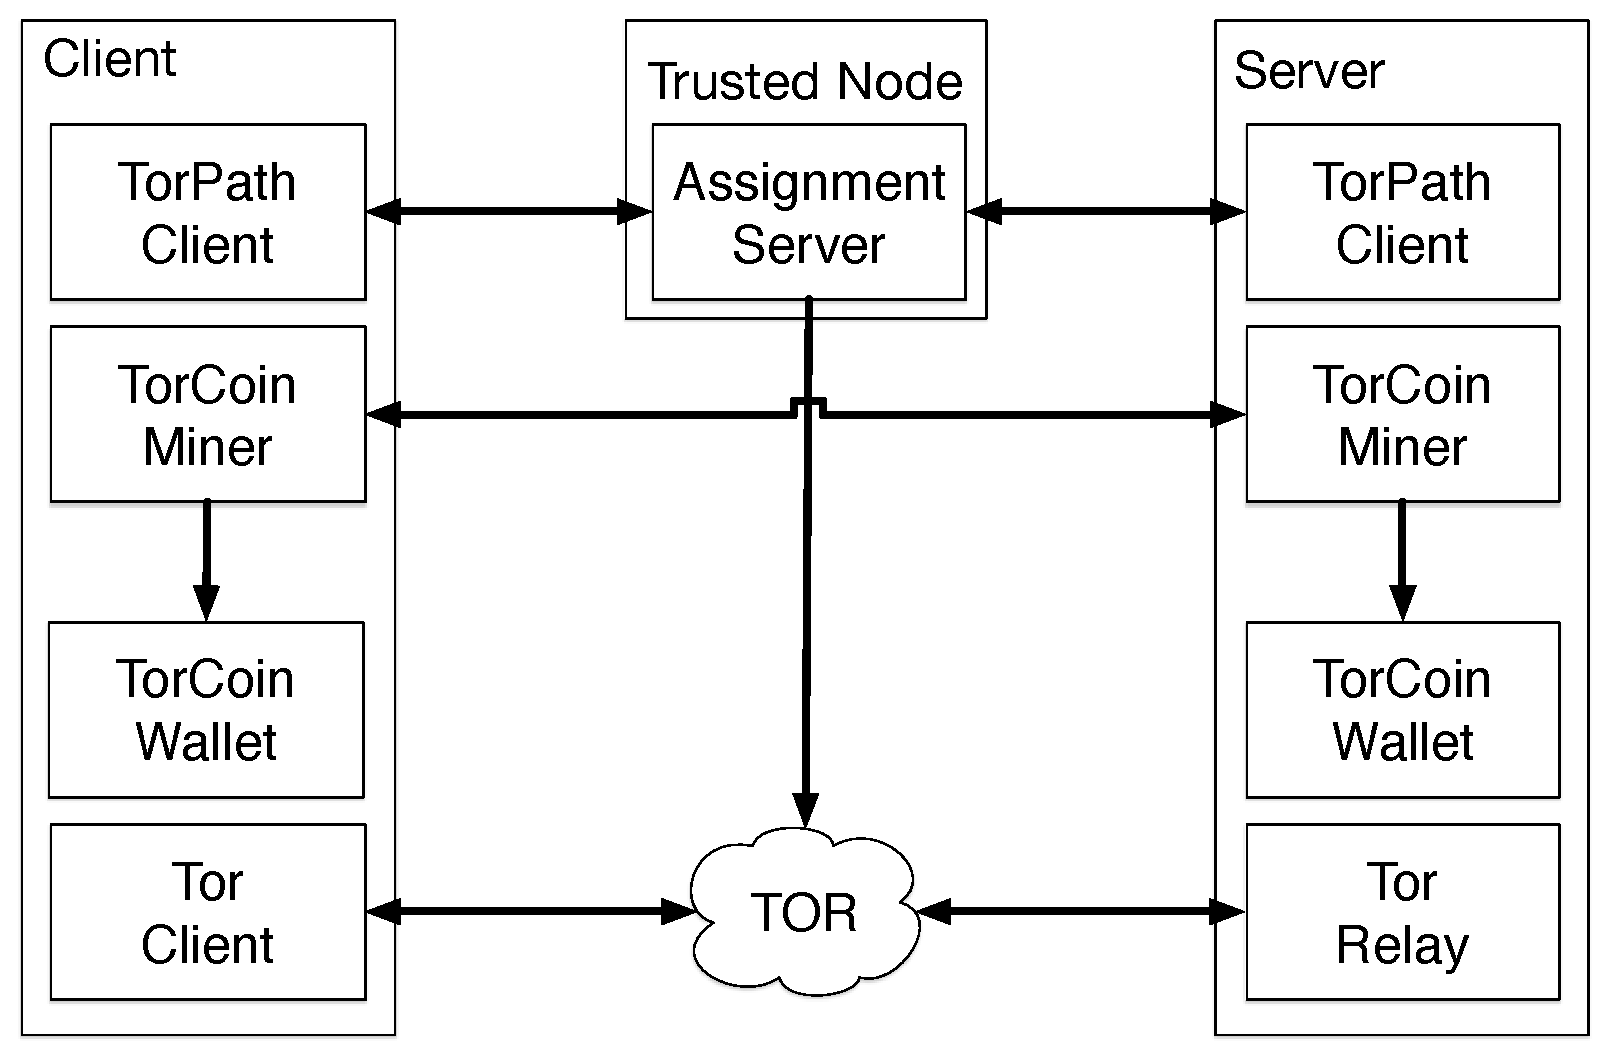
\includegraphics[scale=0.3]{architecture.pdf}
  \caption{High level TorCoin system architecture.}
\end{figure}

We will briefly describe the role of each component in the system. Then, the next two sections will describe the detailed implementations of the TorPath protocol and TorCoin algorithm.

\subsubsection{Assignment Server}
A small set of trusted nodes installs the Assignment Server, in order to override the current Tor directory servers. Groups of assignment servers use the distributed TorPath protocol, described in the next section, to assign circuits to clients and distribute access control lists (ACLs) to relays.

\subsubsection{TorPath Client}
Clients and relays install the TorPath Client to communicate with Assignment Servers, using the TorPath protocol to retrieve circuits (clients) or ACLs (relays).

\subsubsection{TorCoin Miner}
To mine TorCoins, clients and relays that are part of a circuit communicate via the TorCoin miner, which implements the TorCoin algorithm described in the next section.

\subsubsection{TorCoin Wallet}
Since TorCoin is based on the BitCoin protocol, it uses a cryptographic wallet for storage of coins and transactions.

\subsubsection{Tor Client (Unmodified)}
There is no difference in the Tor Client. It connects to relays in the same way as it currently does, but depends on the TorPath client for circuit selection.